\section{\sysname{} Design}
\label{sec:system}

To address the issues with manual policies or application-specific
optimizations, \sysname{} structures adaptation as a set of approximate,
modular, and extensible specifications (\autoref{sec:structure-adapt}). The
well-defined structure allows us to build a generic profiling tool that learns
an accurate relationship---we call it the profile---between bandwidth
consumption and application accuracy (\autoref{sec:automatic-profiling}). The
profile then guides the runtime to react with precision: achieving low latency
and high accuracy when facing insufficient bandwidth
(\autoref{sec:runtime}). \autoref{fig:overview} shows the high-level overview of
\sysname{}.

\begin{figure}
  \centering
  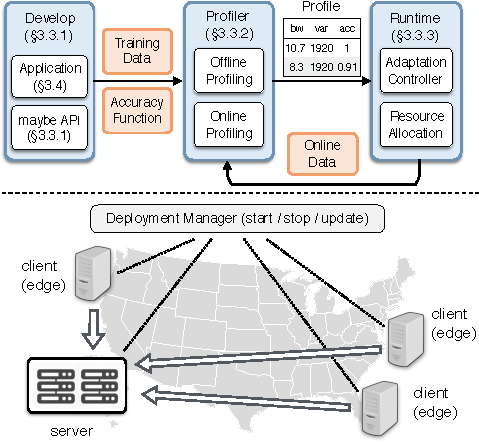
\includegraphics[width=0.9\linewidth]{figures/system.pdf}
  \caption{\sysname{}'s phases: development, profiling, and runtime. \sysname{}
    also manages wide-area deployment.}
  \label{fig:overview}
\end{figure}

\subsection{API for Structured Adaptation}
\label{sec:structure-adapt}

%% Introduce graphs of operators model
Most stream processing systems construct applications as a directed graph of
operators~\cite{toshniwal2014storm, zaharia2013discretized}. Each operator
transforms input streams into new streams. \sysname{} borrows the same
computation model.  \autoref{tab:operators} lists some example operators, such
as \texttt{map} and \texttt{skip}.

To integrate adaptation as a first-class abstraction, \sysname{} introduces
\maybe{} operators that degrade data quality, yielding potential bandwidth
savings.  Our API design has three considerations. $(i)$~To free developers from
specifying exact rules, the API should allow specifications with
options. $(ii)$~To allow combining multiple dimensions, the API should be
modular. $(iii)$~To support flexible integration with arbitrary degradation
functions, the API should take user-defined functions. Therefore, our API is,

\vspace{-2pt}
\begin{lstlisting}
        maybe(knobs: Vec<T>, f: (T, I) => I)
\end{lstlisting}

We illustrate the use of the \texttt{maybe} operator with an example that
quantizes a stream of integers in Rust:

\begin{table*}
  \small
  \centering
  \begin{tabular}{ c r l }
    \toprule
    \multirow{4}{*}{Normal Operators}
    & \textit{map} (f: I $\Rightarrow$ O) & Stream<I> $\Rightarrow$ Stream<O> \\
    & \textit{skip} (i: Integer) & Stream<I> $\Rightarrow$
                                   Stream<I> \\
    & \textit{sliding\_window} (count: Integer, f: Vec<I> $\Rightarrow$ O) & Stream<I> $\Rightarrow$
                                                                            Stream<O> \\
    % & \textit{tumbling\_window} (count: Integer, f: Vec<I> $\Rightarrow$ O) & Stream<I> $\Rightarrow$
    %                                                                          Stream<O> \\
    % & \textit{timed\_window} (time: Duration, f: Vec<I> $\Rightarrow$ O) & Stream<I> $\Rightarrow$
    %                                                                      Stream<O> \\
    & ... & ... \\
    \midrule
    \multirow{5}{*}{Degradation Operators}
    & \textit{maybe} (knobs: Vec<T>, f:  (T, I) $\Rightarrow$ I) & Stream<I> $\Rightarrow$
                                                                 Stream<I> \\
    & \textit{maybe\_skip} (knobs: Vec<Integer>) & Stream<I> $\Rightarrow$ Stream<I> \\
    & \textit{maybe\_head} (knobs: Vec<Integer>) & Stream<Vec<I>{}> $\Rightarrow$
                                                   Stream<Vec<I>{}> \\
    & \textit{maybe\_downsample} (knobs: Vec<(Integer, Integer)>) & Stream<Image> $\Rightarrow$ Stream<Image> \\
    & ... & ... \\
    \bottomrule
  \end{tabular}
  \vspace{0.2em}
  \caption{Stream processing operators in \sysname{}. \texttt{Vec<T>} represents
    a list of elements with type \texttt{T}.}
  \label{tab:operators}
  \vspace{-1em}
\end{table*}

\vspace{-2pt}
\begin{lstlisting}
let quantized_stream = vec![1, 2, 3, 4].into_stream()
    .maybe(vec![2, 4], |k, val| val.wrapping_div(k))
    .collect();
\end{lstlisting}

The snippet creates a stream of integers, chains a degradation operation, and
collects the execution result. In this example, the knob is [2, 4] and the
degradation function performs a wrapping (modular) division where the divisor is
the chosen knob. The knob value modifies the quantization level, affecting the
output: [1, 2, 3, 4] (no degradation), [0, 1, 1, 2] (k=2), or [0, 0, 0, 1]
(k=4). If the stream is then encoded---e.g. run-length encoding as in
JPEG~\cite{wallace1992jpeg}---for transmission, the data size will depend on the
level of degradation.

Based on the \texttt{maybe} primitive, one can implement additional degradation
operators for common data types. For instance, \texttt{maybe\_head} will
optionally take the top values of a list; \texttt{maybe\_downsample} can resize
the image to a configured resolution. \sysname{} provides a number of such
operations as a library to simplify application development
(\autoref{tab:operators}).

With our API, the example mentioned in \autoref{subsec:motivation} can now be
implemented as follows:

\vspace{-4pt}
\begin{lstlisting}
let app = Camera::new((1920, 1080), 30)
    .maybe_downsample(vec![(1600, 900), (1280, 720)])
    .maybe_skip(vec![2, 5])
    .map(|frame| frame.show())
    .compose();
\end{lstlisting}

This snippet first instantiates a \texttt{Camera} source, which produces
\texttt{Stream<Image>} with 1920x1080 resolution and 30 FPS\@. Two degradation
operations follow the source: one that downsamples the image to 1600x900 or
1280x720 resolution, and the other that skips every 2 or 5 frames, resulting in
30/(2+1)=10 FPS or 30/(5+1)= 6 FPS\@. This example then displays degraded
images. In practice, operators for further processing, such as encoding and
transmission, can be chained.

%%% Local Variables:
%%% mode: latex
%%% TeX-master: "../awstream"
%%% End:

%% LocalWords: UDFs Vec quantization quantized quantizes
%% LocalWords: downsample downsamples subsec resize

\subsection{Automatic Profiling}
\label{sec:automatic-profiling}

After developers use \maybe{} operators to specify potential degradation
operations, \sysname{} automatically builds an accurate profile. The profile
captures the relationship between \textit{application accuracy} and
\textit{bandwidth consumption} under different combinations of data degradation
operations. We describe the formalism, followed by techniques that efficiently
perform offline and online profiling.

\para{Profiling formalism.} Suppose a stream processing application has $n$
\maybe{} operators. Each operator introduces a knob $k_i$. The combination of
all knobs forms a \textit{configuration} $c = [k_{1}, k_{2}, ... k_{n}]$. The
set of all possible configurations $\mathbb{C}$ is the space that the profiling
explores. For each configuration $c$, there are two mappings that are of
particular interest: a mapping from $c$ to its bandwidth consumption $B(c)$ and
its accuracy measure $A(c)$. \autoref{tab:notations} summarizes these symbols.

The profiling looks for Pareto-optimal configurations; that is, for any
configuration $c$ in the Pareto-optimal set $\mathbb{P}$, there is no
alternative configuration $c'$ that requires less bandwidth and offers a higher
accuracy. Formally, $\mathbb{P}$ is defined as follows:

{\small \vspace{-1em}
  \begin{equation}
  \mathbb{P} = \{ c \in \mathbb{C} : \{ c' \in \mathbb{C}: B(c') < B(c),
  A(c') > A(c) \} = \varnothing\}
  \label{eq:pareto}
\end{equation}
}%

\begin{table}
  \footnotesize
  \centering
  \begin{tabular}{r l}
    \toprule
    \textbf{Symbol} & \textbf{Description} \\
    \midrule
    $n$ & number of degradation operations \\
    $k_i$ & the \textit{i}-th degradation knob \\
    $c = [k_{1}, k_{2}, ... k_{n}]$ & one specific configuration \\
    $\mathbb{C}$ & the set of all configurations \\
    \midrule
    $B(c)$ & bandwidth requirement for $c$ \\
    $A(c)$ & accuracy measure for $c$ \\
    $\mathbb{P}$ & Pareto-optimal set \\
    \midrule
    $c_i$, $c_{i+1}$, $c_{\max}$ & current/next/maximal configuration at runtime \\
    $R$ & network delivery rate (estimated bandwidth) \\
    $\text{Q}_\text{E}$, $\text{Q}_\text{C}$ & messages when \texttt{Queue} is empty or congested \\
    $\text{R}_\text{C}$ & message when \texttt{Receiver} detects congestion \\
    $\text{AC}_\text{Probe}$ & message when \texttt{AC} requests probing \\
    $\text{S}_\text{ProbeDone}$ & message when \texttt{Socket} finishes probing \\
    \bottomrule
  \end{tabular}
  \vspace{0.3em}
  \caption{Notations used in this paper.}
  \label{tab:notations}
  \vspace{-3em}
\end{table}

Because \sysname{} allows arbitrary functions as the degradation functions, it
does not assume a closed-form relationship for $B(c)$ and $A(c)$. Instead,
\sysname{} takes a data-driven approach: profiling applications with
developer-supplied training data.  We measure $B(c)$ at the point of
transmission. The accuracy $A(c)$ is measured either against the groundtruth, or
the reference results when all degradation operations are off.  We show examples
of knobs, configurations, and accuracy functions when we present applications in
\autoref{sec:implementation}.

\para{Offline Profiling.} We first use an offline process to build a bootstrap
profile (or default profile).  \sysname{} makes no assumptions on the
performance models, and thus evaluates all possible configurations.  While all
knobs form a combinatorial space, the offline profiling is only a one-time
process.  We exploit parallelism to reduce the profiling time.  Without any
\textit{a priori} knowledge, all configurations are assigned randomly to
available machines.

% \para{Offline Profiling.} We first use an offline process to build a bootstrap
% profile (or default profile).  Because \sysname{} supports arbitrary
% degradation operations, we need to evaluate all combinations of the
% configurations offline profiling is a one-time process, \sysname{} currently
% performs an exhaustive evaluation of all configurations in $\mathbb{C}$
% despite all knobs form a combinatorial space. Future work could explore
% statistical methods to build performance models with a smaller number of
% training samples~\cite{venkataraman2016ernest, alipourfard2017cherrypick}.
% \sysname{} exploits parallelism when profiling all configurations.  Without
% any \textit{a priori} knowledge, all configurations are assigned randomly to
% all available machines.

\para{Online Profiling:} \sysname{} supports online profiling to continuously
refine the profile. The refinement handles \textit{model drift}, a problem when
the learned profile fails to predict the performance accurately. There are two
challenges with online profiling.  $(i)$~There are no ground-truth labels or
reference data to compute accuracy. Because labeling data is prohibitively labor
intensive and time consuming~\cite{russell2008labelme}, \sysname{} currently
uses raw data (data without degradation) as the reference. At runtime, if the
application streams raw data, it is used for online profiling. Otherwise, we
allocate additional bandwidth to transmit raw data, but only do so when there is
spare capacity. $(ii)$~Exhaustive profiling is expensive. If the profiling takes
too much time, the newly-learned profile may already be stale. \sysname{} uses a
combination of parallelization and sampling to speed up profiling, as below:

\begin{itemize}[leftmargin=*, topsep=3pt]

\item Parallelization with degradation-aware scheduling. Evaluating each
  configuration takes a different amount of time. Typically, an increase in the
  level of degradation leads to a decrease in computation; for example, a
  smaller FPS means fewer images to process. Therefore, we collect processing
  times for each configuration from offline profiling and schedule online
  profiling with longest first schedule (LFS)~\cite{karger2010scheduling} during
  parallelization.

\item Sampling-based profiling. Online profiling can speed up when we sample
  data or configurations. Sampling data reduces the amount of data to process,
  but at a cost of generating a less accurate profile. When sampling
  configuration, we can evaluate a subset of the Pareto-optimal configurations
  and compare their performances with an existing profile. A substantial
  difference, such as more than \SI{1}{Mbps} of bandwidth estimation, triggers a
  full profiling over all configurations to update the current profile.

\end{itemize}

%%% Local Variables:
%%% mode: latex
%%% TeX-master: "../awstream"
%%% End:

%% LocalWords: ProbeDone th combinatorial runtime parallelization priori
%% LocalWords: LFS mbps groundtruth
\subsection{Runtime Adaptation}
\label{sec:runtime}

At runtime, \sysname{} matches data rate to available bandwidth to minimize
latency and uses Pareto-optimal configurations to maximize accuracy. This
section focuses on the details of our runtime design. We defer the evaluation
and comparisons with existing systems (e.g.\,JetStream) to
\autoref{sec:runtime-adaptation}.

\begin{figure}
  \centering
  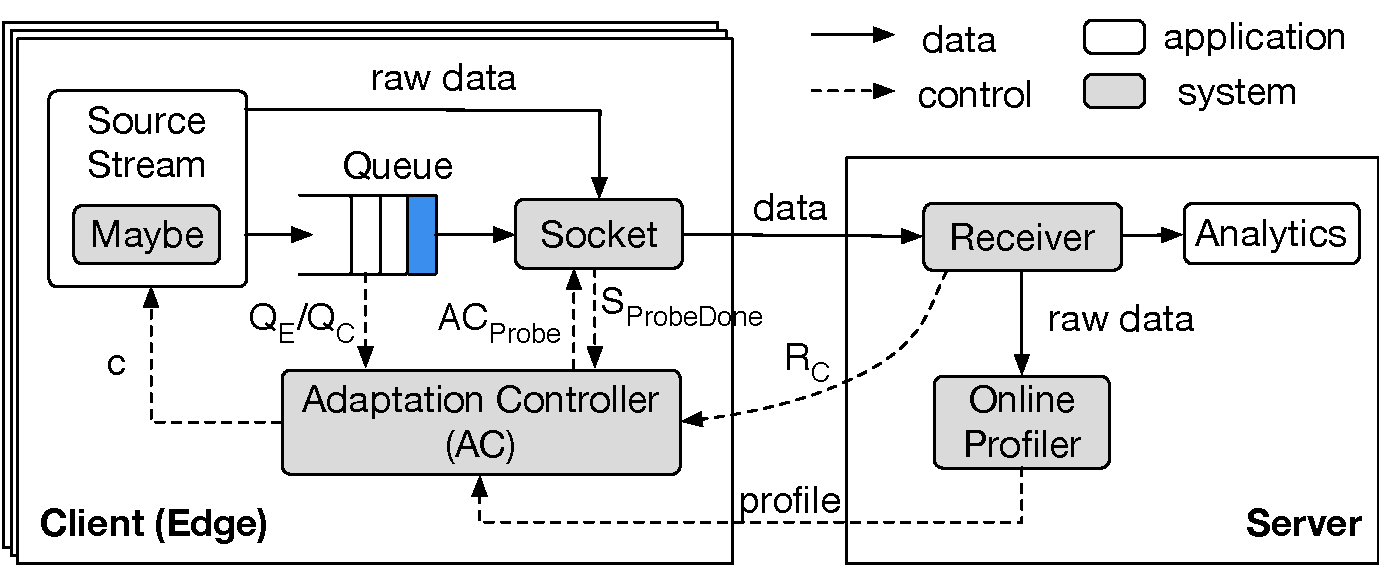
\includegraphics[width=\linewidth]{figures/runtime-adaptation.pdf}
  \caption{Runtime adaptation system architecture.}
  \label{fig:runtime}
\end{figure}

\autoref{fig:runtime} shows our runtime system architecture. \sysname{}
applications' source contains a \texttt{Maybe} module derived from all \maybe{}
operators. This module allows the controller to update the level of
degradation. Data generated by the source is then enqueued to \texttt{Queue} and
subsequently dequeued by \texttt{Socket}, which sends data over the network
using TCP. When the data generation rate exceeds \texttt{Socket}'s departure
rate, the queue grows. In this case, the adaptation controller (AC) queries the
estimated bandwidth from \texttt{Socket} and regulates the source stream by
updating the configuration. After the data is sent through the network,
\texttt{Receiver} delivers data to the application analytics. \texttt{Receiver}
also performs congestion detection and extracts raw data, if it is present.  It
tracks the minimal latency (similar to how BBR tracks
\texttt{RTprop}~\cite{cardwell2017bbr}) and reports sudden application-level
latency spikes to clients as congestion signals (\rc{}). If a new profile is
learned by the online profiler, it is fed back to AC for subsequent adaptation.

\autoref{fig:cc-sm} shows the adaptation algorithm with a state machine model
and \autoref{fig:cc-ex} shows the state transitions with an example. We first
describe all symbols. AC loads the profile and sorts all configurations with an
ascending order of bandwidth demand, resulting in a list
$[c_1, \dots, c_{\max}]$.  These configurations follow a total order:
$c_i < c_j$ if $B(c_i) < B(c_j)$.  We denote the current configuration as $c_i$
and the next $c_{i+1}$.  AC receives messages from other modules: \qe{} when
\texttt{Queue} is empty; $\text{Q}_\text{C}$ when queued items exceed a
threshold; and \rc{} when \texttt{Receiver} detects congestion. AC can query
\texttt{Socket} for delivery rate $R$ (arrow not shown) or request it to probe
($\text{AC}_{\text{Probe}}$) for a target bandwidth, often $B(c_{i+1})$. If
there is no congestion during the probing and $R > B(c_{i+1})$, \texttt{Socket}
sends back \spd{}. Below, we describe each state and transitions.

\begin{figure}
  \begin{subfigure}[t]{\columnwidth}
    \centering
    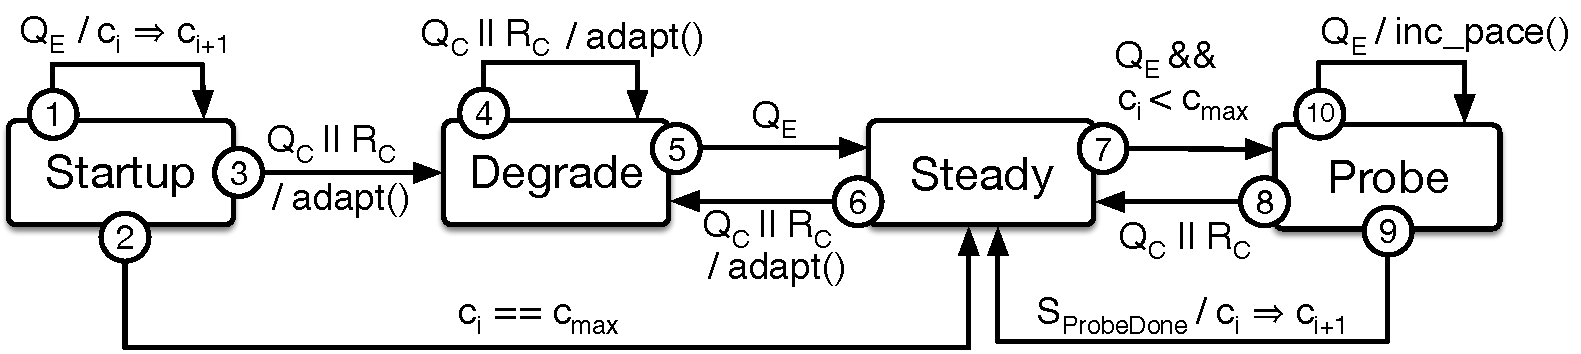
\includegraphics[width=\columnwidth]{figures/cc.pdf}
    \caption{Rate adaptation as a state machine.}
    \label{fig:cc-sm}
  \end{subfigure}
  \vspace{0.5em}
  \\
  \centering
  \begin{subfigure}[t]{\columnwidth}
    \centering
    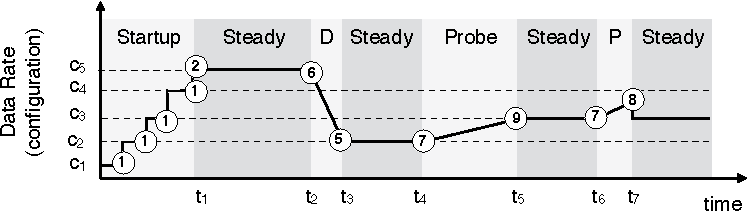
\includegraphics[width=0.9\columnwidth]{figures/cc2.pdf}
    \caption{An example illustrating the adaptation algorithm.}
    \label{fig:cc-ex}
  \end{subfigure}
  \caption{Runtime adaptation algorithm.}
  \label{fig:cc}
\end{figure}

\begin{itemize}[leftmargin=*, topsep=3pt, itemsep=0pt]

\item \textbf{Startup: rapid growth.} \sysname{} starts with $c_1$ and grows the
  rate ($c_i \Rightarrow c_{i+1}$) upon each \qe{}. The growth stops at
  $c_{\max}$ (to \texttt{Steady}) or if it receives \qc{}/\rc{} (to
  \texttt{Degrade}).

\item \textbf{Degrade: reacting to congestion.} Congestion is detected in two
  ways: (1) when \texttt{Queue} grows and exceeds a threshold, AC receives
  \qc{}; (2) when \texttt{Receiver} detects latency spikes, AC receives
  \rc{}. During congestion, AC runs the \texttt{adapt()} procedure by updating
  \texttt{Maybe} with the maximum-allowed $c$ that satisfies $B(c) < \alpha R$,
  where $\alpha \in (0, 1)$ and $R$ is \texttt{Socket}'s current delivery
  rate. A smaller $\alpha$ allows a quicker draining of the queue. After the
  congestion is resolved (\qe{} received), \sysname{} changes to
  \texttt{Steady}.

\item \textbf{Steady: low latency delivery.} \sysname{} achieves low latency by
  spending most of the time in \texttt{Steady}. It changes to \texttt{Degrade}
  when congestion occurs. If $c < c_{\max}$ and it receives \qe{}, AC starts
  \texttt{Probe} to check for more available bandwidth.

\item \textbf{Probe: more bandwidth for a higher accuracy.} Advancing $c_i$
  directly may cause congestion if $B(c_{i+1}) \gg B(c_i)$. To allow a smooth
  increase, AC requests \texttt{Socket} to probe by sending additional traffic
  controlled by \texttt{probe\_gain} (in \texttt{inc\_pace()}, similar to
  BBR~\cite{cardwell2017bbr}). Raw data is used for probing if available,
  otherwise we inject dummy traffic. \sysname{} stops probing under two
  conditions: (1) upon \spd{}, it advances $c_i$; (2) upon \qc{} or \rc{}, it
  returns to \texttt{Steady}. The explicit \texttt{Probe} phase stabilizes
  feedback loop and prevents oscillation.

\end{itemize}


\subsection{Resource Allocation \& Fairness}

In addition to rate adaptation, the profile is also useful for controlling a
single application's bandwidth usage or allocating resources among competing
tasks.

For individual applications, developers can pin-point a configuration for a
given bandwidth or accuracy goal. They can also specify a criterion to limit
effective configurations. For example, \sysname{} can enforce an upper bound on
the bandwidth consumption (e.g.,~do not exceed \SI{1}{Mbps}) or a lower bound on
application accuracy (e.g.,~do not fall below 75\%).

For multiple applications, their profiles allow novel bandwidth allocation
schemes such as utility fairness. Different from resource fairness with which
applications get an equal share of bandwidth, utility fairness aims to maximize
the \textit{minimal} application accuracy. With the profiles, bandwidth
allocation is equivalent to finding proper configuration $c^t$ for application
$t$. We formulate utility fairness as follows:

%% Pick one based on the space

\vspace{-0.5em}
\begin{equation}
  \vspace{-0.5em}
  \label{eq:multitask}
 \underset{c^t}{\max} \; \min({A^t(c^t)})
 \;
 \text{s.t.}
 \;
 \sum_t{B^t(c^t)} < R
\end{equation}

% \begin{equation}
%  \label{eq:multitask}
%  \begin{aligned}
%     & \underset{c^t}{\text{maximize}} & & \min({A^t(c^t)}) & & \\
%     & \text{subject to} & & \sum_t{B^t(c^t)} < R & & \\
%  \end{aligned}
% \end{equation}

Solving this optimization is computationally hard. \sysname{} uses heuristics
similar to VideoStorm~\cite{zhang2017live}: it starts with $c^t_1$ and improves
the application $t$ with the worst accuracy; this process iterates until all
bandwidth is allocated.

%%% Local Variables:
%%% mode: latex
%%% TeX-master: "../awstream"
%%% End:

%% LocalWords: runtime analytics enqueued dequeued TCP JetStream
%% LocalWords: RTprop BBR profiler sm VideoStorm

%%% Local Variables:
%%% mode: latex
%%% TeX-master: "../../thesis"
%%% End:
